\documentclass[letterpaper]{article}
\usepackage[margin=1in]{geometry} % Sets page size and 1-inch margins
\usepackage[svgnames,dvipsnames]{xcolor}   % For a wider range of colors

\usepackage{amsmath} % For math symbols like \lor, \langle, \rangle, \to
\usepackage{array}   % For advanced column specifications
\usepackage{tabularx}% For tables with auto-expanding columns
\usepackage{tikz}
\usetikzlibrary{
    positioning,      % For placing nodes relative to each other (e.g., below=of)
    shapes.geometric, % For shapes like ellipses
    arrows.meta,      % For advanced arrow tips (e.g., Stealth)
    decorations.pathmorphing, % For snake/squiggly lines
    calc              % For coordinate calculations
}

% --- GLOBAL STYLE DEFINITIONS FOR DFD ---
\tikzset{
    % A shape for logical connectives
    connective_node/.style={
        rectangle, rounded corners=5pt, draw=black!80, fill=black!10,
        inner sep=5pt, thick, align=center
    },
    % A shape for Introduction Rules
    intro_rule_node/.style={
        rectangle, rounded corners=5pt, draw=black!80, fill=Teal!20,
        inner sep=5pt, thick, align=center
    },
    % A shape for Elimination Rules
    elim_rule_node/.style={
        rectangle, rounded corners=5pt, draw=black!80, fill=BurntOrange!20,
        inner sep=5pt, thick, align=center
    },
    % A shape for abstract propositions
    proposition_node/.style={
        ellipse, draw=black!80, fill=Violet!15,
        inner sep=3pt, align=center
    },
    % A shape for concrete proof terms
    proof_node/.style={
        ellipse, draw=black!80, fill=Green!15,
        inner sep=3pt, align=center
    },
    % Arrow styles with color
    input_arrow/.style={-Stealth, solid, thick, draw=blue!70!black},
    output_arrow/.style={double, double distance=1.5pt, -Stealth, solid, thick, draw=ForestGreen!80!black},
    proves_arrow/.style={-Stealth, decorate, decoration={snake, segment length=6pt, amplitude=1pt}, thick, draw=orange!90!black}
}

% --- Define and measure boxes to get widths for tabularx ---
\newlength{\orheaderwidth}
\settowidth{\orheaderwidth}{\textbf{Or} : Prop $\to$ Prop $\to$ Prop}
\addtolength{\orheaderwidth}{1em}


\begin{document}

\begin{figure}[h!]
\centering
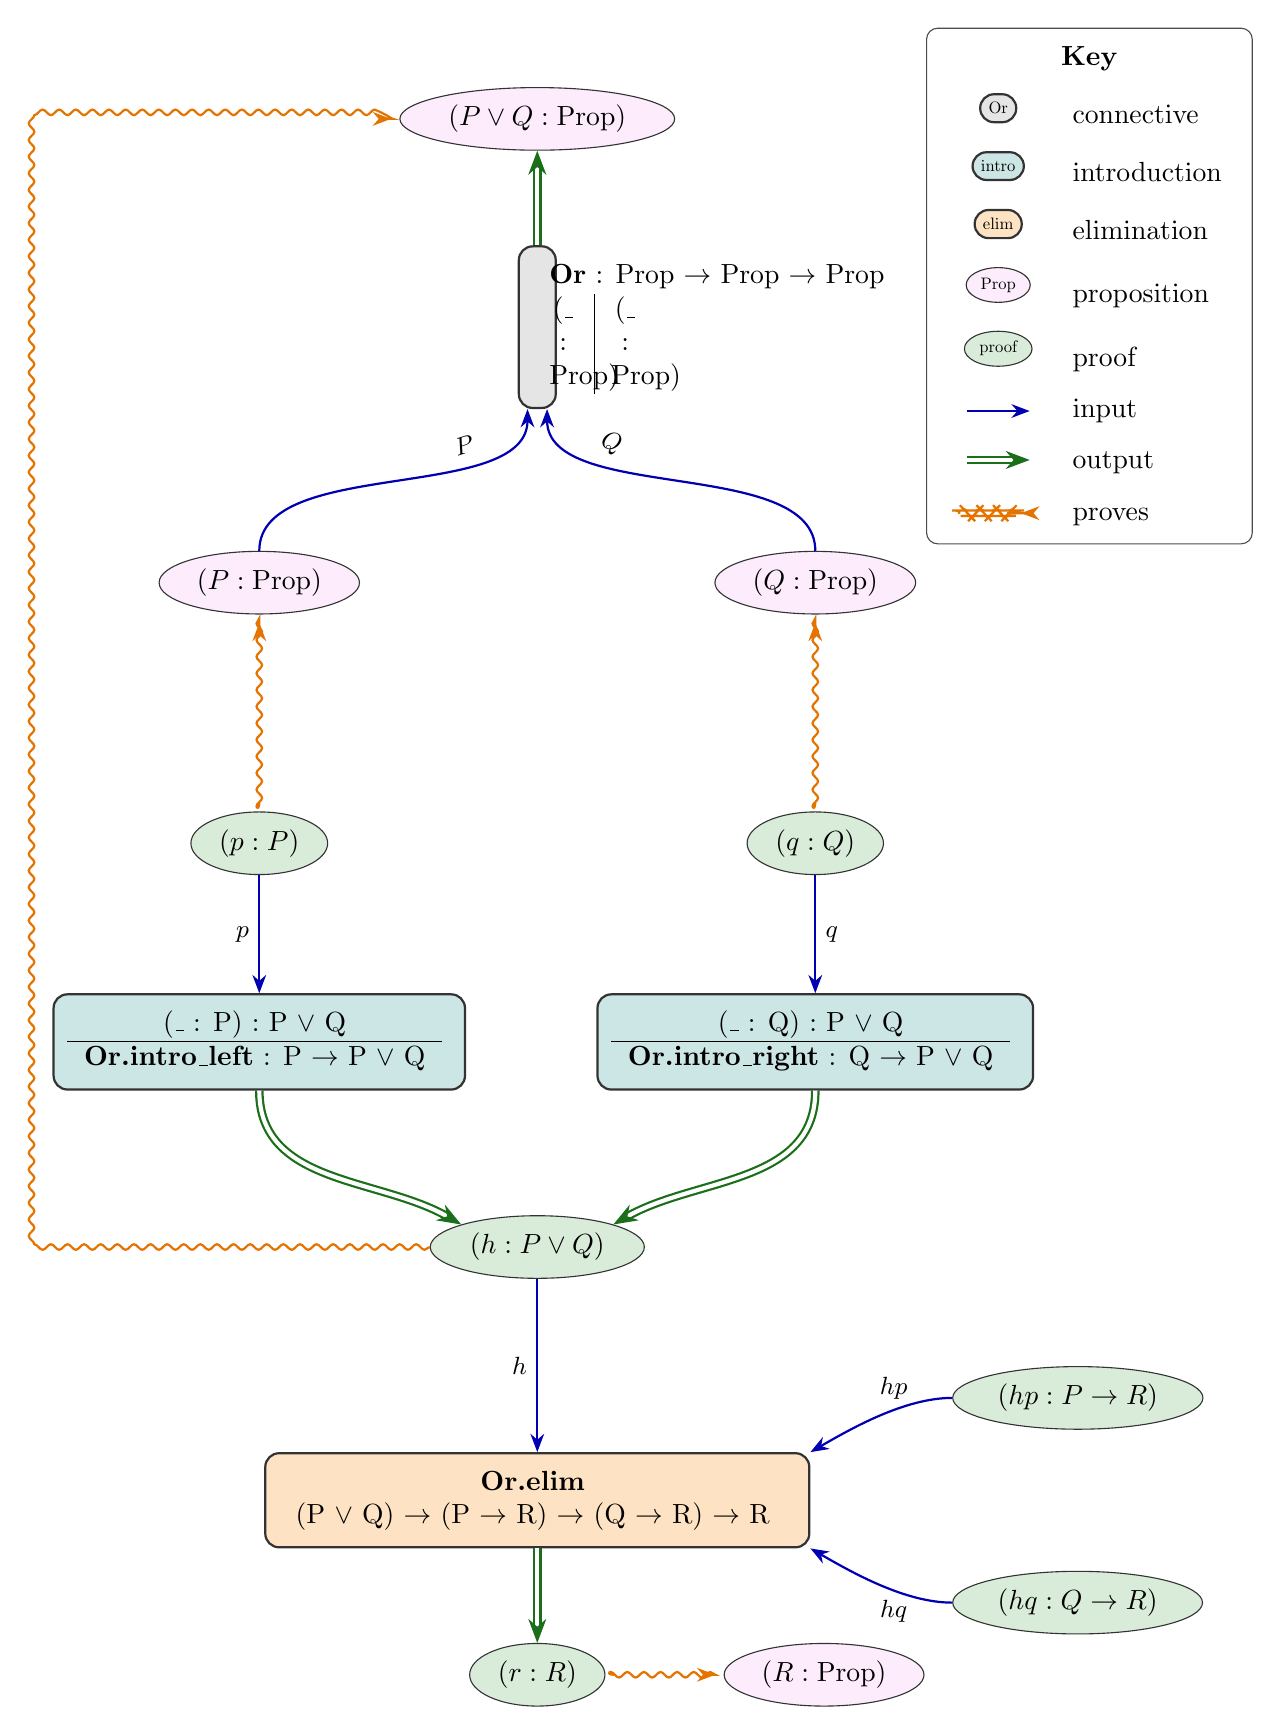
\begin{tikzpicture}[node distance=2.2cm and 2.5cm]

% --- NODE DEFINITIONS FOR "OR" DIAGRAM ---

% Top layers
\node[proposition_node] (P_prop) {$(P : \text{Prop})$};
\node[proposition_node] (Q_prop) [right=4.5cm of P_prop] {$(Q : \text{Prop})$};

\node[connective_node, above=1.8cm of $(P_prop.north)!.5!(Q_prop.north)$] (or_box) {
    \begin{tabularx}{\orheaderwidth}{>{\centering\arraybackslash}X|>{\centering\arraybackslash}X}
        \multicolumn{2}{c}{\textbf{Or} : Prop $\to$ Prop $\to$ Prop} \\ \hline
        (\_ : Prop) & (\_ : Prop)
    \end{tabularx}
};

\node[proposition_node] (P_or_Q_prop) [above=1.2cm of or_box] {$(P \lor Q : \text{Prop})$};

% Introduction Layer - nodes are now closer to their types above
\node[proof_node] (p_P) [below=2.5cm of P_prop] {$(p : P)$};
\node[proof_node] (q_Q) [below=2.5cm of Q_prop] {$(q : Q)$};

\node[intro_rule_node, below=1.5cm of p_P] (or_inl) {
    \begin{tabular}{c}
    (\_ : P) : P $\lor$ Q \\ \hline
    \textbf{Or.intro\_left} : P $\to$ P $\lor$ Q
    \end{tabular}
};
\node[intro_rule_node, below=1.5cm of q_Q] (or_inr) {
    \begin{tabular}{c}
    (\_ : Q) : P $\lor$ Q \\ \hline
    \textbf{Or.intro\_right} : Q $\to$ P $\lor$ Q
    \end{tabular}
};

% Elimination Layer
\node[proof_node] (h_P_or_Q) [below=2.2cm of $(or_inl)!.5!(or_inr)$] {$(h : P \lor Q)$};

\node[elim_rule_node, below=2.2cm of h_P_or_Q] (or_elim) {
    \begin{tabular}{c}
    \textbf{Or.elim} \\
    (P $\lor$ Q) $\to$ (P $\to$ R) $\to$ (Q $\to$ R) $\to$ R
    \end{tabular}
};

% The hypothesis proofs are positioned closer to the elim node.
\node[proof_node] (hp_P_to_R) [right=1.8cm of or_elim, yshift=1.3cm] {$(hp : P \to R)$};
\node[proof_node] (hq_Q_to_R) [right=1.8cm of or_elim, yshift=-1.3cm] {$(hq : Q \to R)$};

\node[proof_node] (result_R) [below=1.2cm of or_elim] {$(r : R)$};
\node[proposition_node] (R_prop) [right=1.5cm of result_R] {$(R : \text{Prop})$};


% --- BEAUTIFUL EDGE ROUTING ---
\draw[output_arrow] (or_box) -> (P_or_Q_prop);
\draw[input_arrow] (P_prop.north) to[out=90, in=-90, looseness=0.8] node[pos=0.7, sloped, above, font=\small] {$P$} ($(or_box.south west)!.5!(or_box.south)$);
\draw[input_arrow] (Q_prop.north) to[out=90, in=-90, looseness=0.8] node[pos=0.7, sloped, above, font=\small] {$Q$} ($(or_box.south)!.5!(or_box.south east)$);

\draw[input_arrow] (p_P) -> node[left, font=\small] {$p$} (or_inl.north);
\draw[input_arrow] (q_Q) -> node[right, font=\small] {$q$} (or_inr.north);

\draw[output_arrow] (or_inl.south) to[out=-90, in=150] (h_P_or_Q.north west);
\draw[output_arrow] (or_inr.south) to[out=-90, in=30] (h_P_or_Q.north east);

% Input arrows are now short, direct, and unambiguous.
\draw[input_arrow] (h_P_or_Q) -> node[left, font=\small] {$h$} (or_elim);
\draw[input_arrow] (hp_P_to_R) to[out=180, in=30, looseness=0.8] node[pos=0.4, above, font=\small] {$hp$} (or_elim.north east);
\draw[input_arrow] (hq_Q_to_R) to[out=180, in=-30, looseness=0.8] node[pos=0.4, below, font=\small] {$hq$} (or_elim.south east);
\draw[output_arrow] (or_elim) -> (result_R);

% Type/proves arrows are now shortened.
\draw[proves_arrow, shorten <=3pt, shorten >=3pt] (p_P) -> (P_prop);
\draw[proves_arrow, shorten <=3pt, shorten >=3pt] (q_Q) -> (Q_prop);
\draw[proves_arrow, shorten <=3pt, shorten >=3pt] (result_R) to[out=0, in=180] (R_prop);

% The crisp polyline, guaranteed to be outside the diagram and fit the page.
\coordinate (outset_point) at ($(P_prop.west)+(-1.5cm,0)$);
\draw[proves_arrow, shorten >=3pt] (h_P_or_Q.west) -- (outset_point |- h_P_or_Q.west) -- (outset_point |- P_or_Q_prop.west) -- (P_or_Q_prop.west);


% --- FINAL LEGEND ---
% Repositioned to be safely anchored to Q_prop, avoiding any overlap.
\node (legend) [draw=black!70, rounded corners, inner sep=5pt, above right=0.2cm and 0.5cm of Q_prop] {
    \begin{tabular}{cl}
    \multicolumn{2}{c}{\textbf{Key}} \\[1.5ex]
    \tikz{\node[connective_node, scale=0.6] {Or};} & connective \\[1.5ex]
    % --- CORRECTED LINE ---
    % The typo '1.sex' has been fixed to '1.5ex'.
    \tikz{\node[intro_rule_node, scale=0.6] {intro};} & introduction \\[1.5ex]
    \tikz{\node[elim_rule_node, scale=0.6] {elim};} & elimination \\[1.5ex]
    \tikz{\node[proposition_node, scale=0.6] {Prop};} & proposition \\[1.5ex]
    \tikz{\node[proof_node, scale=0.6] {proof};} & proof \\[1.5ex]
    \tikz{\draw[input_arrow] (0,0.1) -- (0.8,0.1);} & input \\[1.5ex]
    \tikz{\draw[output_arrow] (0,0.1) -- (0.8,0.1);} & output \\[1.5ex]
    \tikz{\draw[proves_arrow] (0,0.1) -- (0.8,0.1);} & proves \\
    \end{tabular}
};

\end{tikzpicture}
\caption{The algebra of logical disjunction. The Or function builds the proposition
$P \lor Q$. There are two introduction rules: $Or.intro\_left$ takes a proof of $P$ 
to prove $P \lor Q$, while $Or.intro\_right$ uses a proof of $Q$. To use a proof of 
a disjuction, the $Or$ elimination rule takes a proof $h$ of $P \lor Q$ along with 
a proof that if $P$ is true, so is $R$, and a proof that if $Q$ is true, then so is
$R$. These two proofs together show that if either of $P$ or $Q$ is true, then so is
$R$. In plain English, if you know either $P$ or $Q$ happened and you know that $R$
will happen in either case (case analysis) then $R$ will happen ($R$ is true).}\label{fig:tikz_diagram_or_final_bugfix_v2}
\end{figure}

\end{document}